\documentclass[aps,prl,twocolumn,superscriptaddress,amsmath,amssymb,floatfix]{revtex4-2}
\usepackage{graphicx}
\usepackage{xcolor}
\usepackage{bm}
\usepackage[colorlinks=true,allcolors=blue]{hyperref}
\newcommand{\tbd}[1]{\textcolor{red}{[#1]}}
\renewcommand{\topfraction}{0.95}
\renewcommand{\bottomfraction}{0.95}
\renewcommand{\textfraction}{0.05}
\renewcommand{\floatpagefraction}{0.85}

\begin{document}

\title{On the richness of metamaterials generated by recursive cell division}

\author{Alexei Vazquez}
\email{alexei@nodeslinks.com}
\affiliation{Nodes \& Links Ltd, Salisbury House, Station Road, Cambridge, CB1 2LA, UK}

\date{\today}

\begin{abstract}
% PRL limit: 600 characters
Recursive cell division generates network metamaterials with a wide range of effective
refractive index $n$. Across division rules, $n$ is capped by the pin-jointed
architecture and the homogenised band closes at the weakest-span resonance. Random
cut angles give high $n$ at high density; cutting through the cell centroid removes
slender spans and gives the widest band at high $n$. Balanced divisions reach low $n$. In
three dimensions plate and strut divisions are near-affine and $n$ stays low. Grading the
cut angle at fixed density routes a shock around a protected component, halving the force
on it.
\end{abstract}

\maketitle

% ---------------------------------------------------------------------------
\paragraph*{Introduction.}
Scale-rich (SR) metamaterials~\cite{both2026}, a recent example of irregular
metamaterial networks~\cite{wytock2026}, are grown one ligament at a time: a ligament
nucleates at a uniform random point and angle and grows until it meets the existing
structure, with thickness $\lambda_t=\lambda_0t^{-\alpha}$ for the $t$-th ligament.
Their unit cells reach effective refractive indices $1.5\le n\le8.3$, against
$1.0\le n\le1.9$ for square and hexagonal lattices, and an SR Luneburg lens focuses a
plane wave~\cite{both2026}. Geometrically the SR construction is Cowan's iterated cell
division: the cell holding the point, chosen in proportion to its area, is cut by a
chord~\cite{cowan2010,vazquez2026sr}; with axis-parallel cuts and no thickness it is a
STIT (Mondrian) tessellation~\cite{nagel2005}.

\begin{figure}[b]
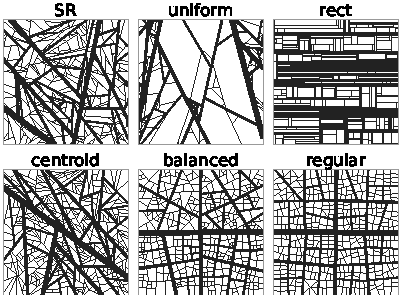
\includegraphics[width=\columnwidth]{fig1.pdf}
\caption{\label{fig:rules}Recursive divisions of the square, $T=400$ ligaments, line
width $\propto t^{-1/2}$ ($\alpha=1/2$). SR: cell $\propto$ area, uniform point, uniform
angle. \emph{uniform}: cell chosen uniformly. \emph{rect}: axis-parallel cuts.
\emph{centroid}: cut through the centroid. \emph{balanced}: centroid cut perpendicular to
the major axis. \emph{regular}: as \emph{balanced}, largest cell first.}
\end{figure}

Cowan's construction defines a whole family of recursive divisions. A rule specifies
which cell is cut, where the cut passes, and at what angle. Changing these choices
produces materials that range from scale-rich hierarchies to nearly uniform cells. All
of them are generated just as simply, and all accept the same thickness hierarchy.

In the long-wavelength regime a cellular solid of relative density $\bar\rho$ and
effective stiffness tensor $C$ carries quasi-longitudinal waves with velocity
$v(\hat{\bm k})$, the largest eigenvalue of the Christoffel matrix
$\Gamma_{ik}=C_{ijkl}\hat k_j\hat k_l$ divided by $\bar\rho$~\cite{auld1973}. The
effective refractive index $n(\hat{\bm k})=c_0/v(\hat{\bm k})$, with $c_0$ the velocity
in the constituent, is the design variable of gradient-index (GRIN) devices such as
elastic Luneburg lenses~\cite{tol2017,aguzzi2022}. A GRIN device realises a prescribed
profile $n(\bm r)$ with isotropic cells, and works up to the frequency at which the
homogenised index of its weakest cell fails. The design question is therefore which
cell gives the widest band at each required index; cells generated by different rules
can be tiled together.

Here we ask a more general question: which structure among Cowan's recursive divisions
is best for elastic-wave control? We compare six division rules, from scale-rich to
nearly uniform, with the SR thickness hierarchy. In two dimensions they are ligament
frames and in three dimensions plate and strut networks. For each rule we compute $n$,
its isotropy and the band over which it holds, from Bloch waves on periodic tilings, and
compare the rules at equal $n$. Random cut angles through the cell centroid give the
widest band over most of the index range, and balanced divisions extend it to low index. Finally, we
show that grading the cut angle at fixed density routes a shock around a protected
component.

% ---------------------------------------------------------------------------
\paragraph*{What sets the range of $n$.}
Before comparing rules, it helps to know which values of $n$ any architecture can reach
and what makes $n$ large. A porous material is at most as stiff as its constituent
diluted by the density: this is the Voigt bound~\cite{hill1952}, $C\le\bar\rho\,C^{0}$.
Waves are therefore never faster in the architecture than in the constituent, and
$n\ge1$ for every design, with equality for ligaments aligned with the wave. There is no
universal upper limit: $n$ diverges as the structure approaches a mechanism. A wide range
of $n$ alone is therefore not a useful figure of merit, since any rule that comes close
to a mechanism reaches it, at the price of isotropy and bandwidth. This is why we compare
rules at equal $n$.

A large $n$ needs a soft longitudinal modulus. A longitudinal wave compresses the
material, so it probes $C_{11}\sim K+G$ rather than the Young modulus. A honeycomb, soft
in $E$ but stiff in the bulk modulus $K$~\cite{deshpande2001}, keeps $n\simeq1.9$ at
every density. A network of T-junctions is soft in both. Its stiffness has two parts.
With pin joints the network carries load by stretching alone, with a modulus
$C^{\rm pin}=\bar\rho\,s$ that vanishes for a mechanism~\cite{maxwell1864}. Rigid joints
add the bending of the ligaments, as in stiff fibre networks~\cite{wilhelm2003,head2003},
which grows with their thickness $\lambda$. Hence
\begin{equation}
n^{-2}=s+c\,(\lambda/\ell)^{q},\qquad n\le n_{\max}=s^{-1/2},
\label{eq:ceiling}
\end{equation}
where $\ell$ is a typical span and $c$ and $q$ characterise the architecture. The
pin-jointed architecture caps the index, and slender ligaments bring $n$ close to the
cap.

% ---------------------------------------------------------------------------
\paragraph*{Recursive divisions.}
We compare six rules (Fig.~\ref{fig:rules}). Cells are picked in proportion to area
(SR), uniformly among the cells (\emph{uniform}), or largest first (\emph{regular}). The
cut passes through a uniform point of the cell (SR, \emph{uniform}, \emph{rect}) or
through its centroid (\emph{centroid}, \emph{balanced}, \emph{regular}). Its direction is
uniform (SR, \emph{uniform}, \emph{centroid}), axis-parallel (\emph{rect}), or
perpendicular to the major axis of the cell (\emph{balanced}, \emph{regular}). The
\emph{uniform} rule produces a broader distribution of cell sizes than SR. The
\emph{balanced} and \emph{regular} rules produce nearly equal cells. Every rule uses the
SR thickness $\lambda_t=\lambda_0t^{-\alpha}$, with $\lambda_0$ set by $\bar\rho$.

Each cell holds $T=10^3$ ligaments, modelled as an Euler--Bernoulli frame with rigid
joints ($E_0=\rho_0=1$). The square boundary is generation zero of the division, so the
material is a periodic tiling of cells whose frames are shared with their
neighbours~\cite{both2026}; we tile by mirror images, which makes the tiling exactly
periodic. Periodic homogenisation gives $C$, and the Christoffel equation gives
$n(\hat{\bm k})$ and the isotropy $\eta_n=\min n/\max n$. Bloch waves along $x$ and $y$
give the band edge $\omega_h$, the highest frequency at which the longitudinal branch
keeps its plane-wave character and its index within $10\%$ of the static value. The
clamped cell gives the lowest local resonance $\omega_1$. Frequencies are in units of
$c_0/L$, with $L$ the cell size. We scan $\alpha\in[0,1]$ and $\bar\rho\in[0.03,0.4]$,
and use square, triangular, honeycomb and Voronoi lattices as references.

% ---------------------------------------------------------------------------
\begin{figure}[tb]
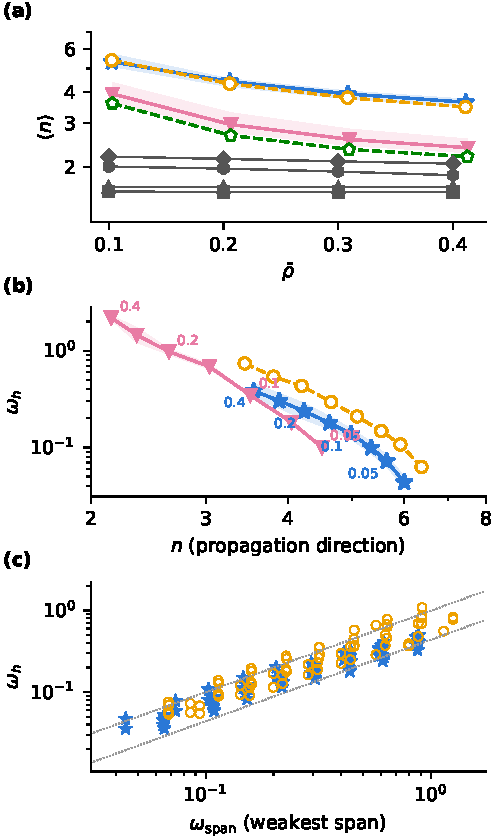
\includegraphics[width=\columnwidth]{fig2.pdf}
\caption{\label{fig:2d}Two dimensions, periodic tilings, $T=10^3$, $\alpha=0$. Stars: SR;
circles: \emph{centroid}; inverted triangles: \emph{balanced}; pentagons: \emph{regular}; grey
squares, triangles, hexagons and diamonds: square, triangular, honeycomb and Voronoi
lattices. (a)
Direction-averaged index against density (frame included). Lines: geometric mean over
four realisations; bands: their range (SR, \emph{balanced}); grey: reference lattices.
\emph{Centroid} coincides with SR and \emph{regular} with \emph{balanced}: the cut angle,
not the cut position, sets the index. (b) Bloch band edge $\omega_h$ (units $c_0/L$) at fixed index along the
propagation direction: each density scan (four realisations, $x$ and $y$) is interpolated
at fixed $n$; lines: mean of $\ln\omega_h$, bands: $\pm$ one standard error. (c) $\omega_h$
against the weakest-span prediction $\omega_{\rm span}$ of Eq.~(\ref{eq:span}), every
cell; dotted lines: clamped ($\omega_h=\omega_{\rm span}$) and pinned
($\omega_h=(\pi/4.730)^2\omega_{\rm span}$) spans.}
\end{figure}

\paragraph*{Index from density and architecture.}
The SR cells span $1.70\le n_x\le6.76$, consistent with the reported
$1.5$--$8.3$~\cite{both2026} (Fig.~\ref{fig:2d}a). The square, triangular, honeycomb and
Voronoi lattices give $n_x=1.41$, $1.72$, $1.9$--$2.1$ and $2.1$. Two quantities set
$n$. The first is density: at $\alpha=0$ the direction-averaged SR index falls from
$\langle n\rangle=5.3$ at $\bar\rho=0.1$ to $3.7$ at $\bar\rho=0.4$. The hierarchy
exponent matters less: at $\bar\rho=0.2$, $\alpha=0,0.25,0.5,0.75,1$ gives
$n_x=4.04,2.84,2.31,2.24,2.36$. The second is the architecture, and within it the
distribution of cut angles. At equal density the rules with random cut angles are softer:
at $\bar\rho=0.4$, SR and \emph{centroid} give $\langle n\rangle=3.7$ and $3.5$, whereas
\emph{balanced} and \emph{regular}, which cut perpendicular to the long axis, give $2.4$
and $2.2$. Where the cut passes matters little: SR and \emph{centroid} agree within
$4\%$ at every density.
The balanced rules are more isotropic, with $\eta_n=0.78$ against $0.67$ for SR at
$\bar\rho=0.2$.

\paragraph*{The weakest span sets the band.}
The lowest local resonance is the flexural mode of the weakest span between junctions.
A span of length $\ell_s$ and thickness $\lambda_s$ has its lowest mode at
\begin{equation}
\omega_s=\beta^2\frac{\lambda_s}{\sqrt{12}\,\ell_s^2}\,c_0 ,
\label{eq:span}
\end{equation}
with $\beta=\pi$ for pinned ends and $\beta=4.730$ for clamped
ends~\cite{aguzzi2022}. The prediction $\omega_{\rm span}=\min_s\omega_s$ with clamped
ends has no free parameter. It tracks $\omega_1$ over three decades, with a correlation
of $0.979$ between $\ln\omega_1$ and $\ln\omega_{\rm span}$ over all 480 cells. The ratio
$\omega_1/\omega_{\rm span}$ lies between $0.44=(\pi/4.730)^2$, the pinned limit, and
$0.70$: junctions rotate, so the weakest span is partly clamped. The Bloch band edge
follows the same prediction (Fig.~\ref{fig:2d}c), with correlations $0.97$, $0.94$ and
$0.97$ for SR, \emph{centroid} and \emph{balanced}: the long-wavelength description fails
where the weakest span resonates. The prefactor $\omega_h/\omega_{\rm span}$ is $0.63$ for
SR and $0.79$ for \emph{centroid}, between the pinned and clamped limits, but $0.31$ for
\emph{balanced}. In a balanced division many spans have nearly the same length; resonating
together, they form a band whose lower edge lies below the frequency of a single span.

\paragraph*{Index from architecture keeps the band.}
Equations~(\ref{eq:ceiling}) and (\ref{eq:span}) together fix the trade-off. A target
$n$ requires a thickness $\lambda=\ell\,[(n^{-2}-s)/c]^{1/q}$, and the band edge grows
with $\lambda$. Eliminating $\lambda$,
\begin{equation}
\omega_h(n)\simeq\Omega\,\bigl(n^{-2}-n_{\max}^{-2}\bigr)^{1/q},\qquad
\Omega=\frac{\beta^2}{\sqrt{12}}\,\frac{\ell}{\ell_{\max}^2}\,c^{-1/q},
\label{eq:tradeoff}
\end{equation}
where $\ell_{\max}$ is the weakest span. The band scale $\Omega$ is set by how uniform
the spans are; the ceiling $n_{\max}$ sets where the band collapses. Fitted to the
clamped resonances, Eq.~(\ref{eq:tradeoff}) describes the \emph{balanced} and
\emph{regular} divisions within $1$--$9\%$, and the scale-rich divisions within about
$30\%$, where the weakest span varies from realisation to realisation. Pinning the joints of the periodic tilings gives the index ceiling of
each rule: $n_{\max}=4.8$--$8.1$ for SR (depending on the realisation), $5.4$--$7.9$ for
\emph{centroid}, and $5.6$--$5.8$ for \emph{balanced} and \emph{regular}. The coefficient
$c$ differs more: at $\bar\rho=0.4$ the bending term of \emph{balanced} is six times that
of SR. A balanced division therefore reaches a high index only with slender ligaments,
close to its ceiling, where the band collapses. The random-angle divisions reach the same
index at high density, far below their ceiling, with stubby ligaments. The measured
exponent $q\simeq0.7$--$1.1$, smaller than the value $2$ of pure bending, shows that
stretching and bending are coupled, as near the rigidity point of fibre networks.

The Bloch band edges at fixed index (Fig.~\ref{fig:2d}b) give the answer. Below
$n\simeq2.7$ only the balanced divisions are available, with $\omega_h$ up to $1.5$. At
$n=3$, \emph{balanced} and \emph{centroid} tie ($\omega_h=0.65$) and SR trails ($0.37$).
From $n\simeq3.5$ upwards \emph{centroid} gives the widest band: $\omega_h=0.50$, $0.33$
and $0.23$ at $n=3.5$, $4$ and $5.5$, against $0.35$, $0.25$ and $0.09$ for
\emph{balanced} and $0.22$, $0.15$ and $0.17$ for SR, with standard errors of
$15$--$25\%$. SR overtakes \emph{balanced} only above $n\simeq4.5$ and matches
\emph{centroid} only near $n=5$. The two random-angle rules have the same index at a
given density (Fig.~\ref{fig:2d}a) and differ in where the cut passes. A cut through a
uniform point often removes a sliver, leaving a short span next to a long one; a cut
through the centroid does not. The random angles provide the index, and the centroid cut
removes the slender spans that close the band.

% ---------------------------------------------------------------------------
\begin{figure}[tb]
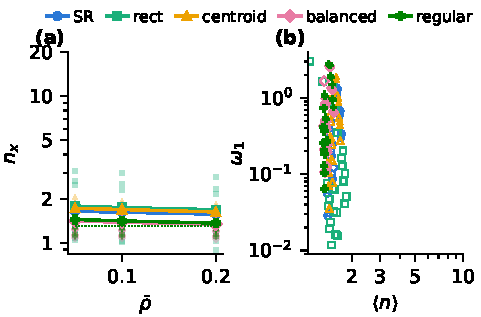
\includegraphics[width=\columnwidth]{fig3.pdf}
\caption{\label{fig:3d}Three dimensions, divisions of the cube, $T=300$. Solid lines and
filled symbols: plates; dashed lines and open symbols: struts. Stars: SR; circles:
\emph{centroid}; inverted triangles: \emph{balanced}; pentagons: \emph{regular}; squares:
\emph{rect}. (a) Direction-averaged index against density, $\alpha=0$. (b) Lowest local
resonance $\omega_1$ (units $c_0/L$) against $\langle n\rangle$, $\alpha\in\{0,1/2,1\}$.}
\end{figure}

\paragraph*{Three dimensions: the ceiling is low.}
A recursive division of the cube cuts convex polyhedra by planes, so the material is a
closed-cell network of plates~\cite{both2026}; its edges form an open-cell network of
struts. We use the same rules, with isotropic, axis-parallel or major-axis normals, and
$T=300$ plates per cell. Plates are meshed with triangles that conform across T-junction
lines~\cite{shewchuk1996} and modelled by constant-strain membranes and discrete
hinges~\cite{grinspun2003} ($\nu_0=0.3$); struts are three-dimensional Euler--Bernoulli
beams. The moduli converge to 1--2\% under mesh refinement, change by less than $1\%$
from $T=300$ to $600$, and agree within 1--3\% between affine and periodic boundaries. The
\emph{uniform} rule is excluded: its plates are thicker than they are wide.

In three dimensions the ceiling of Eq.~(\ref{eq:ceiling}) is low (Fig.~\ref{fig:3d}). A
convex cell with rigid planar faces is rigid, so, as in periodic plate
lattices~\cite{berger2017,tancogne2018}, membranes alone carry the load. With bending
switched off, SR plates give $n_{\max}=1.73$ and \emph{balanced} plates $1.58$; the full
model gives $1.71$ and $1.54$ at $\bar\rho=0.05$. Over the scan, $\alpha\in\{0,1/2,1\}$
and $\bar\rho\in\{0.05,0.1,0.2\}$, every rule stays within $1.32\le\langle n\rangle\le1.84$.
The open-cell struts run straight through the junctions, which also makes them rigid:
$2.3\le\langle n\rangle\le3.7$ for every rule, nearly independent of density. Without a
high-index window, the uniform spans decide: at equal $n$ the balanced divisions have the
higher band edge, $\omega_1=1.30$ against $0.20$ for SR plates at $\langle n\rangle\simeq1.5$
and $0.22$ against $0.06$ for struts at $\langle n\rangle\simeq3.6$.

% ---------------------------------------------------------------------------
\begin{figure}[tb]
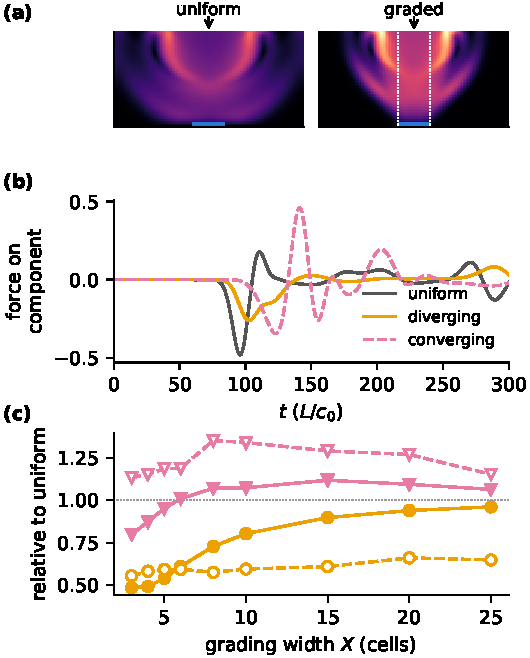
\includegraphics[width=\columnwidth]{fig4.pdf}
\caption{\label{fig:shock}Shock routing in a lattice insert at fixed density
($\bar\rho=0.2$; homogenised cells of the cut-angle family). A half-sine pulse of
duration $20\,L/c_0$ hits the top of a $60\times30$-cell slab on a rigid base above a
component (blue). (a) Displacement amplitude at $t=100\,L/c_0$ for the uniform slab
($\kappa=0$) and the diverging grading ($\kappa$ rising from 0 to 1 within $X=5$ cells of
the axis, dotted). (b) Force on the component. (c) Peak force (filled) and transmitted
impulse (open) relative to the uniform slab against $X$; circles: diverging, inverted
triangles: converging grading.}
\end{figure}

\paragraph*{Application: routing a shock at fixed density.}
The cut angle tunes $n$ at fixed density: at $\bar\rho=0.2$, tilting each centroid cut
from perpendicular to the long axis ($\kappa=0$, the \emph{balanced} rule) to a uniform
angle ($\kappa=1$, \emph{centroid}) raises $n$ from $2.94$ to $4.41$ continuously, with
a spread of $0.01$--$0.15$ between realisations; with density, $2.4\le n\le5.5$ within one
family. Mass and density then stay uniform while the wave speed varies, which suits a
load-bearing part. Graded truss lattices already redirect impacts~\cite{radi2024}. Protective inserts for
electronics and equipment face sub-millisecond shocks, short enough for the wavelength to
be comparable to the part. We
model a lattice insert on a rigid base protecting a component, hit directly above it
(Fig.~\ref{fig:shock}), with homogenised cells and the same polymer loss in every cell;
less than $1\%$ of the pulse spectrum lies above the band edge of the cells used. Rays
bend towards high index, so a low-index column above the component flanked by high-index
cells routes the stress around it. Within $X=5$ cells of the axis, this grading halves the
peak force on the component and cuts the transmitted impulse by a quarter, at unchanged
mass. The reverse grading focuses the shock, raising the impulse by $40$--$80\%$. Steeper
gradients approach the limit of the homogenised description, set by the cell size.

% ---------------------------------------------------------------------------
\paragraph*{Conclusions.}
The family of recursive divisions is richer than its scale-rich member. The index comes
from two sources, slender ligaments and a soft architecture; the pin-jointed architecture
caps it, and the weakest span sets the band over which it holds. Index from slenderness
costs bandwidth; index from architecture does not. Random cut angles make the
architecture soft, so the scale-rich division reaches high index at high density, which
is the regime of the SR Luneburg lens~\cite{both2026}. Cutting through the centroid
instead of a random point keeps that index and removes the slender spans, giving the
widest band from $n\simeq3.5$ upwards; balanced divisions reach the low-index range.
In three dimensions plate and strut divisions are near-affine, the ceiling is low, and
the uniform spans of balanced divisions keep the higher bandwidth. The cut angle is a
continuous design variable: it tunes $n$ by $1.4$--$1.5\times$ at fixed density, which
routes a shock around a protected component at unchanged mass. Above the
band edge, local resonances open gaps~\cite{liu2000}, a separate design problem in which
the broad span spectrum of a scale-rich division may be an asset.

\begin{acknowledgments}
All code is available at \url{https://github.com/av2atgh/scalerich/tree/master/beyond}.
The calculations were assisted by Claude Opus~5.5, an AI assistant developed by Anthropic.
Nodes \& Links Ltd provided support in the form of salary for Alexei Vazquez but did not
have any additional role in the conceptualization of the study, the analysis, the decision
to publish or the preparation of the manuscript.
\end{acknowledgments}

\bibliography{refs}

% ---------------------------------------------------------------------------



\end{document}
